\documentclass{article}
\usepackage{fullpage}
\usepackage{moreverb}
\usepackage{graphicx}

\begin{document}

\title{Manual of Disambiguation}
\author{Ye (Edward) Sun}
\date{August, 2011}
\maketitle

\section{Overview}

The source code is an implementation of authorship 
disambiguation algorithm described by Vetle
Torvik et al 2009. While it is originally designed 
for the disambiguation of inventors in the United
States Patent and Trademark Office (USPTO) database, 
minor modifications in the source file can
provide solutions for problems of the similar kind.

The algorithm uses Bayesian theorem to calculate the 
probability of match between two records based
on the comparison between the two records in significant 
attributes such as names, geographical location and companies, 
etc. The algorithm includes three major steps: 1. Blocking,
2. Training, and 3. Disambiguation.  The details of each 
step are described in the following sections.

The source code is written in C++ and uses many features 
of C++, such as polymorphism, template, STL library, etc. 
Therefore, a fairly good understanding of C++ is expected 
to fully understand the code. The code also outsources 
IBM CPLEX for quadratic programming. Import and export of the
disambiguation result may need some APIs of SQL/SQLite. 
The code is compiled in Linux by GNU gcc/g++/make.


\section{Work Flow}

\subsection{Schematic}


\begin{figure}
\begin{center}
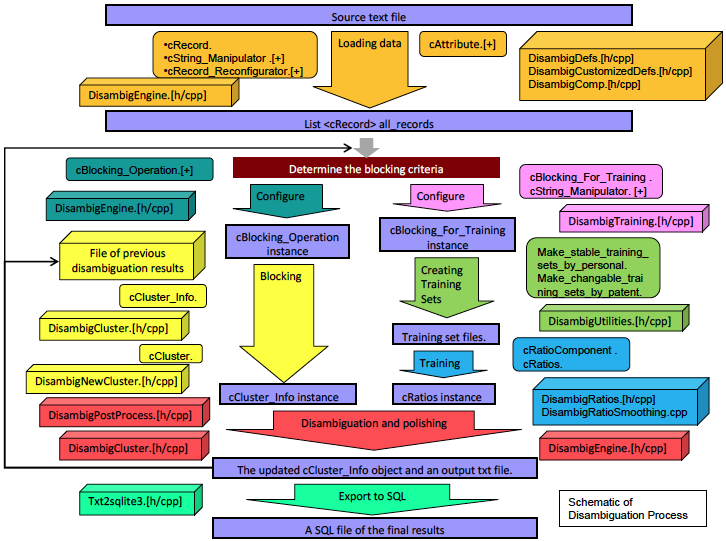
\includegraphics[width=6in]{images/disambiguation_workflow.png}
\caption{Workflow.}
\label{fig:workflow}
\end{center}
\end{figure}



This is a schematic of the whole disambiguation process. 
Each array represents one step, with the
square box of identical color representing the source 
code files that implements the step, and the round
box of identical color representing the necessary 
definitions of relevant classes and/or functions.


The disambiguation is an iterative process: 
the result of previous disambiguation serves as the input of
the next round disambiguation. For each round of disambiguation, 
there are three major steps: blocking, training and disambiguation.

\subsection{Blocking}

Blocking of records is the first step of disambiguation. 
The whole point of blocking is to avoid most
unnecessary comparisons without much accuracy loss. Records 
of similar attributes are blocked
together since they are likely to be a match. Because the 
aim of disambiguation is individual inventors,
the most significant attributes – names – are 
usually adopted as the blocking rules. It is critical to
remember that ONLY records within the same blocks are 
compared and thus disambiguated.


Iterative blocking in a permissive way is applied in the 
disambiguation, because it is assumed that after each round 
of disambiguation, blocks are well disambiguated and thus 
similar and/or more stringent blockings are meaningless. 
For example, the first round of blocking is exact 
first names + exact last names, the second can 
be first 5 characters of first names + first 8 characters 
of last names, and the third round can be first 
3 characters of first names + first 5 characters of last names.


\subsection{Training}

The point of training is to obtain the ratios database for 
similarity profiles based on training sets.

\subsubsection{Similarity Profiles}

Similarity profiles are defined as multi-dimensional variables 
that describe the similarity of two records. Each record has 
many attributes, such as first name, last name, assignee, street, 
city, country, etc. Similarity profiles are selected attributes 
that are believed to be influential in pairwise comparisons; thus, 
they are decided by users and can be different in each round of 
disambiguation. For example, similarity profiles in the first round 
of disambiguation can be “first name + last name + assignee + 
city”, while those in the second round can be “ last name + 
assignee + street ”. Each attribute in a similarity profile is 
given a score to evaluate the similarity of the attribute from the
comparison of the two records. The score is discrete and is usually 
non-negative integers. Scoring of each attribute is totally 
user-defined, and, conceptually, has to be fully understood by users.
Similarity profiles refer to the multi-dimensional integers obtained 
from the comparison.



\subsubsection{Training sets}

Training sets contain pairs of records that are believed 
with high confidence to be either match or
non-match. In the USPTO patent inventor disambiguation, 
there are four training sets:

\begin{enumerate}

\item match pairs to train personal information based 
on patent information: this set is created by selecting 
record pairs belonging to the same blocks and having at 
least two common coauthors.

\item non-match pairs to train personal information based 
on patent information: this set is created by
selecting record pairs that share the same patent id but 
different author sequence of that patent.

\item match pairs to train patent information based on 
personal information: this set is created by
selecting record pairs that share exact rare names.

\item non-match pairs to train patent information based on 
personal information: this set is created by
selecting record pairs whose names are both rare and different.

\end{enumerate}


\subsubsection{Ratios database}


The ratio value of a given similarity profile, or R-value, 
is defined as the frequency of the similarity profile in the 
match set divided by the frequency of the same similarity 
profile in the non-match set. Ratios database, therefore, 
is the mapping of all possible similarity profiles to 
their corresponding r-values. In the patent disambiguation, 
personal information is assumed to be independent from patent
information, so r-value of a similarity profile is the 
multiple of the r-value of the personal information
part of the similarity profile and that of the patent 
information part of it. By using the four training sets
described above, the ratios database can be obtained. Usually 
the ratios database is implemented as a binary search tree. 
Since it is likely that some similarity profiles are not 
observed in match or non-match sets, interpolation and 
extrapolation of those profiles become necessary. Moreover, the
similarity profiles are assumed to be monotonic. Quadratic 
programming is adopted to accomplish the monotonicity 
enforcement, the interpolation and the extrapolation.


\subsection{Disambiguation}


\subsubsection{Clusters}

The smallest unit of disambiguation is a cluster, 
which contains one or more records. A cluster is
interpreted as a unique inventor. The ultimate 
goal of disambiguation is to finalize clusters 
and their components.


\subsubsection{Probability of Match}

When two records are compared to find out the probability 
of match, their similarity profiles are calculated first 
by comparing relevant attributes. Then the corresponding 
r-value is looked up from the ratios database. Finally, the 
Bayesian theorem is applied to get the final probability 
of match, with the help of a priori probability which 
is block-dependent.



\subsubsection{Cluster-based Disambiguation}

During disambiguation, clusters belonging to the same 
blocks are compared. No inter-block cluster comparisons 
would happen. When two clusters are compared, their 
component records are compared exhaustively to find the 
interactive force between the two clusters. The sum of 
the interactive probabilities is compared to internal 
probabilities of both clusters. If the comparison passes a
predetermined threshold, the two clusters are determined 
as of a same inventor and are merged together. The process 
continues independently within each block until no merge 
can happen. Once all blocks are disambiguated, the 
disambiguation process of the current round ends.


\section{Configuration}


\subsection{Prerequisites}


\begin{itemize}

\item A high-end workstation (usually 8 CPUs and 
24G RAM). 24G RAM is probably the minimum memory 
requirement. Since multi-threading is supported, 
more CPUs generally reduce time cost.

\item Linux ( Ubuntu, Fedora or other compatibles )

\item GCC/G++ (4.0 or higher)

\item IBM CPLEX

\item SQLite3 (3.6 or higher) (This is not mandatory 
but necessary if one needs to out put the result to
a sqlite3 database).

\end{itemize}


\section{Configuration and Compilation of Executables}


\subsection{Configure IBM CPLEX}

IBM CPLEX package for academia is usually free for download 
and use. Trial versions will not work as limitations apply. 
Follow the instructions to install. Pay attention to the 
architecture (32/64 bit).


\subsubsection{Configure SQLite3}

SQLite3 is a public domain, light weight SQL database engine. 
Download from website and install.


\subsubsection{Configure Makefile}

Edit the file \texttt{makefile} in the source code package. 
Things include

\begin{itemize}

\item The path of IBM CPLEX library and header files 
(pay attention to architecture.)

\item The path of SQLite3 library and header files

\item System libraries and header files (math library, 
pthread library, etc).

\item Optimization flags (optional).

\end{itemize}



\subsubsection{Compile}

In the command line, in the directory where the 
file makefile is, type \texttt{make}
Source codes will compile automatically. A successful 
compilation will generate several executables, namely
\texttt{exedisambig} and \texttt{txt2sqlite3}.
The former is the main disambiguation program, and the 
latter is the executable that dumps the disambiguation 
result into sqlite3 databases. Errors in compilation are 
usually caused by incorrect configurations in 
the \texttt{makefile} file. If necessary, type 
\texttt{make clean} to remove all the newly built 
object files, and \texttt{make} to rebuild.


\subsection{Configuration of Disambiguation}

The disambiguation is configured by two parts: 
the disambiguation engine and the blocking rules.


\subsubsection{Engine Configuration}

The configuration of the disambiguation engine
includes the following items:

\begin{itemize}

\item Working directory: the directory where all the intermediary 
and final files will be saved.

\item Original CSV File: the source database of disambiguation in 
text format, which is usually exported from a SQL database. 
The first line of the file consists of names of each
attribute/column, and the rest lines are data.

\item Number of threads: the number of maximum threads to 
allow multi-threading of the program. Usually it is set to 
be the number of CPUs in the computer.

\item  Generate stable training sets: match and non-match 
training sets from rare names are usually very stable. Therefore, 
if those training sets already exist, this switch can be set 
to false. However, since the creation of the stable 
training sets generally does not take too much time,
it is usually recommended to be \texttt{true}.


\item Use available ratios database: this switch controls 
whether or not training should take place. Since training is 
usually somewhat time-costly (~4 hours), this switch can be 
set to \texttt{true} if training is unnecessary, such as 
when debugging. But generally this option should be set to false.

\item Thresholds: the thresholds series to determine whether 
or not two records are a match should be set in a permissive way, 
such as $0.99$, $0.98$, $0.95$. The reason to do this is to allow most
similar records conglomerate first, which can help improve the accuracy.

\item Necessary attributes: This option selects those necessary 
attributes to load into the memory from the original CSV file, 
because not all the data in the original CSV file need to be loaded.
These necessary attributes should be exactly the same as those 
appearing in the first line of the CSV file.

\item Adjust prior by frequency: This option controls the evaluation 
of the priori probability for each block. It is an option that 
should always set to be true unless modification of the code
occurs after thorough understanding of the code.

\item Debug mode: this switch indicates whether the program is 
for debugging or not. Set to \texttt{false} if a normal 
disambiguation is desired. In debug mode, the program will 
look for the debug configuration file debug\_block\_x.txt 
in the working directory, where x is the current round
of disambiguation. The debug configuration file contains all 
the specified blocks that are of interest, and the program only 
disambiguates those blocks.

\item Number of training pairs: the maximum of pairs of records 
obtained for training. Usually set to 10 million.

\item Starting round: this number specifies the round of 
disambiguation to start with.

\item Starting file: this string specifies the file of previous 
disambiguation result from which the disambiguation starts. If the
starting round is 1, the starting file just needs to be a valid
location in the file system, because it will be automatically 
created or overwritten.


\item Postprocess after each round: the switch determines whether 
or not post-processing should be applied after each round of 
disambiguation. It can be either true or false,
although true is recommended.

\end{itemize}

\subsubsection{Blocking Configuration}


The blocking configuration file determines the blocking 
rules and the similarity profile components
for each round of disambiguation. It is in the format of:

\begin{verbatim}
[ Round X ]

Attribute Name 1: String Manipulation parameters
…
Attribute Name M: String Manipulation parameters
Active Similarity Attributes: attribute names of similarity profile components.

[ Round Y ]

Attribute Name 1: String Manipulation parameters
…
Attribute Name N: String Manipulation parameters
Active Similarity Attributes: attribute names of similarity profile components.
\end{verbatim}


In the current engine, a typical example is:

\begin{verbatim}
[ Round 5 ]

Firstname: 1 : 0 , 3 , true
Middlename: 1 : 0 , 0 , false
Lastname: 0 : 0, 5, true
ACTIVE SIMILARITY ATTRIBUTES: Firstname, Middlename, Lastname, Latitude, Coauthor,
Assignee
\end{verbatim}


This means that the blocking identification for round 5 is
created from three attributes:

\begin{itemize}

\item First name: the raw data is read from the index 1 position
of the first name attribute object (see more details in source codes),
and is truncated from the index 0 position of the string for a
maximum length of 3 characters in a forward direction ( left to right ).

\item Middle name: the raw data is read from the index 1 position
of the middle name attribute object (see more details in source codes),
and is truncated from the index 0 position of the string for a
maximum length of 0 characters in a backward direction ( right to left ).

\item Last name: the raw data is read from the index 0 position of
the last name attribute object (see more details in source codes),
and is truncated from the index 0 position of the string for a
maximum length of 5 characters in a forward direction ( left to right ).
And the components of similarity profiles are: first name, middle name,
last name, latitude (geographical location), coauthor, assignee (company).

\end{itemize}

\subsection{Export Disambiguation Results}

The results of disambiguation can be exported to a
SQLite database by running the \texttt{txt2sqlite3}
executable file.



\section{Implementation Details}


\subsection{Data Structure}


The disambiguation engine is designed in an object-oriented
way. The key concepts in the whole engine include:


\begin{itemize}

\item Attributes: conceptualized as the information in each
column in the database. The attribute class has a complicated
hierarchy and thus requires much more understanding. As for the
implementation, each CONCRETE attribute class has multiple
pointers to data strings. See more details in the source code.

\item Records: a vector of attributes representing a full 
record in the database. More strictly, each
record contains a vector of pointers to attributes.

\item Clusters: conceptualized as a unique inventor having
multiple records. Each cluster contains a list of
pointers to records.

\end{itemize}


The following picture shows the data structure of the disambiguation.



%\begin{figure}
%\begin{center}
%\includegraphics{images/algorithm.pdf}
%\caption{An Algorithm.}
%\label{fig:algorithm}
%\end{center}
%\end{figure}


\begin{figure}
\begin{center}
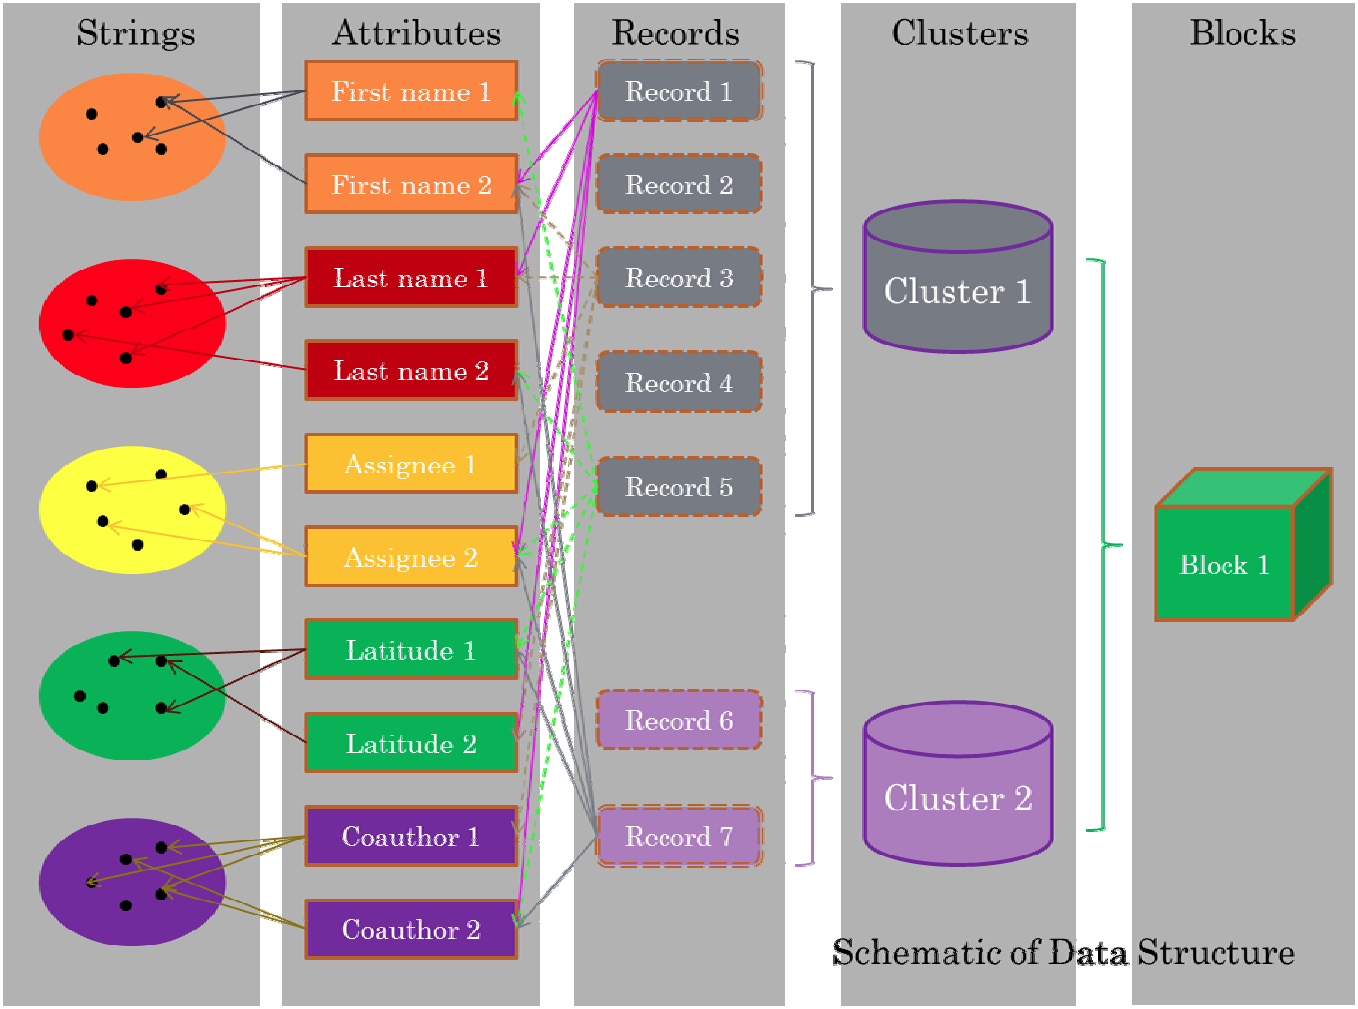
\includegraphics[width=4in]{images/disambiguation_data_structure.png}
\caption{Data structure.}
\label{fig:datastructure}
\end{center}
\end{figure}


\subsection{Customization of Attributes}


The attribute class has several layers of inheritance, 
each of which implements some more functionality and thus 
becomes more concrete. At the  very low level of the 
hierarchy, there are several modes to choose. Ideally one 
only needs to pick up a mode to inherit if a concrete class 
is supposed to be defined. It is also the class creator's 
responsibility to know and to define (or override) the 
following data members and member functions for a 
given concrete class:

\begin{itemize}

\item Class name: the name of the concrete class.

\item Class name specifier string: the name specifier
of the concrete class, which can be used to
retrieve data from the original data file.

\item Class group: the training group of the class, 
such as personal side, patent side, or none.

\item Name specifiers of interactive classes: the 
specifiers of the classes that is necessary for the
current class in order for a viable comparison definition.

\item Number of interactive classes: the number of 
interactive classes.

\item Maximum value: the maximum score of the comparison 
function of the class.

\item Compare: the comparison function of the class.

\item Other functions if necessary.

\end{itemize}

Here is a typical example of the customization of the 
Firstname attribute and the Latitude attribute.

For Firstname:

\begin{itemize}

\item Class name: cFirstname. This class has no interaction 
with other classes and thus simply inherits from the mode 
\texttt{cAttribute\_Single\_Mode<cFirstname>}.

\item Class name specifier string: “Firstname”. 
This is exactly the same as the one in the original
database.

\item Class group: \texttt{Personal}. First name is in the 
personal information side.

\item Name specifiers of interactive classes: {} (empty).

\item Number of Interactive classes: 0

\item Maximum value: 4. The rating is user-defined and has to
be consistent with the comparison function.

\item Compare: Override the parent class definition.

\item Other functions:

\item \texttt{split\_string}: defines how the data is extracted 
from the original database and stored in the
class object.

\item exact\_compare: defines how the exact
comparison function works.

\end{itemize}

For Latitude:

\begin{itemize}

\item Class name: cLatitude. This class has interaction with several 
other attributes, so it inherits from 
\texttt{cAttribute\_Interactive\_Mode<cLatitude, cLatitude\_Data>},
where \texttt{cLatitude\_Data} contains the real data and inherits 
from \texttt{cAttribute\_Singe\_Mode<cLatitude\_Data>}.

\item Class name specifier string: Latitude.

\item Class group: Patent

\item Name specifiers of interactive classes:
{Longitude, City, Country}

\item Number of interactive classes: 3

\item Maximum value: 5.

\item Compare: Overridden.

\end{itemize}


\subsection{Customization of Cluster Comparisons}

Comparison between two clusters, a critical part of
disambiguation, includes several configurable
steps that can be very influential to the results.
When two clusters are compared:

\begin{itemize}

\item  The two representatives of the clusters are compared
to get a post-probability. If the probability does not pass
a minimum screening threshold, the clusters are judged to be of
different inventors and should not merge. The comparison of
the clusters stops here.

\item If the probability passes the minimum threshold, then:

\begin{itemize}

\item Another threshold, dependent on the features of the
clusters, is calculated and will be used as a caliber in the
further disambiguation of the two clusters. The threshold
depends on the cohesions of the two clusters, the career
gap between the clusters, the number of common locations
between the clusters, etc.

\item A priority queue of a given size is created. The size
of the queue depends on the size of both clusters. The larger
the clusters, the larger the queue size.

\item Exhaustive comparisons between members of the two
clusters are performed, and the results are fed into the
priority queue in the following manner.

\end{itemize}

\item If the priority queue is not full, the new result fills into the queue.

\item If the queue is full, the new result is compared with the lowest value in the
queue.

\item If the new result is greater than the lowest value, and the lowest
value is less than the caliber threshold, then the new result simply
replaces the lowest value in the priority queue.

\item If the new results is less than the lowest value but greater than the
caliber threshold, the new result is added to the priority queue.

\item If the new result is less than the lowest value and also less than the
caliber threshold, discard the new result.

o The average value of the priority queue is then calculated after the exhaustive
comparisons finish. If the average is greater than the caliber threshold, the two
clusters are labeled as of a same inventor and will be followed by a merge of the
clusters; otherwise, the comparison of the clusters stops here.

\item If the clusters are labeled as a merge, the two clusters 
will merge into a new bigger cluster, with the previously calculated 
average value of the priority queue as its new cohesion value
(or with-in-cluster density). A new representative of the new 
cluster will be decided later.

\end{itemize}



Therefore, the customization of the cluster comparisons can be in:

\begin{itemize}

\item The screening threshold

\item The caliber threshold

\item The size of the priority queue

\item The way to calculate the new cohesion value (the with-in-cluster density)

\end{itemize}


\appendix


\section{Output files}




\begin{itemize}
\item \texttt{final.txt}
\item \texttt{final.txt.pplog}
\item \texttt{invpat.csv}
\item \texttt{match\_cons2.txt}
\item \texttt{match\_cons.txt}
\item \texttt{network\_1.txt}
\item \texttt{network\_2.txt}
\item \texttt{network\_3.txt}
\item \texttt{network\_4.txt}
\item \texttt{network\_5.txt}
\item \texttt{network\_6.txt}
\item \texttt{newmatch\_1.txt}
\item \texttt{newmatch\_2.txt}
\item \texttt{newmatch\_3.txt}
\item \texttt{newmatch\_4.txt}
\item \texttt{newmatch\_5.txt}
\item \texttt{newmatch\_6.txt}
\item \texttt{postprocesslog\_1.txt}
\item \texttt{postprocesslog\_2.txt}
\item \texttt{postprocesslog\_3.txt}
\item \texttt{postprocesslog\_4.txt}
\item \texttt{postprocesslog\_5.txt}
\item \texttt{postprocesslog\_6.txt}
\item \texttt{prior\_saved\_1.txt}
\item \texttt{prior\_saved\_2.txt}
\item \texttt{prior\_saved\_3.txt}
\item \texttt{prior\_saved\_4.txt}
\item \texttt{prior\_saved\_5.txt}
\item \texttt{prior\_saved\_6.txt}
\item \texttt{ratio\_1.txt}
\item \texttt{ratio\_2.txt}
\item \texttt{ratio\_3.txt}
\item \texttt{ratio\_4.txt}
\item \texttt{ratio\_5.txt}
\item \texttt{ratio\_6.txt}
\item \texttt{stat\_patent\_1.txt}
\item \texttt{stat\_patent\_2.txt}
\item \texttt{stat\_patent\_3.txt}
\item \texttt{stat\_patent\_4.txt}
\item \texttt{stat\_patent\_5.txt}
\item \texttt{stat\_patent\_6.txt}
\item \texttt{stat\_personal\_1.txt}
\item \texttt{stat\_personal\_2.txt}
\item \texttt{stat\_personal\_3.txt}
\item \texttt{stat\_personal\_4.txt}
\item \texttt{stat\_personal\_5.txt}
\item \texttt{stat\_personal\_6.txt}
\item \texttt{tset02\_stable.txt}
\item \texttt{tset05\_1.txt}
\item \texttt{tset05\_2.txt}
\item \texttt{tset05\_3.txt}
\item \texttt{tset05\_4.txt}
\item \texttt{tset05\_5.txt}
\item \texttt{tset05\_6.txt}
\item \texttt{xset01\_1.txt}
\item \texttt{xset01\_2.txt}
\item \texttt{xset01\_3.txt}
\item \texttt{xset01\_4.txt}
\item \texttt{xset01\_5.txt}
\item \texttt{xset01\_6.txt}
\item \texttt{xset03\_stable.txt}

\end{itemize}

\end{document}
